\subsection{Introducci\'on} 

Cada participante de una competencia debe cruzar un puente dando saltos de tabl\'on en tabl\'on, con la limitaci�n de que pueden saltar como m\'aximo una cantidad fija de tablones por vez. Sin embargo algunos de estos tablones est\'an rotos. El objetivo del ejercicio es dar un algoritmo que nos devuelva un recorrido por los tablones del puente el cual sea m�nimo en la cantidad de saltos requeridos para poder cruzarlo con una complejidad temporal de \Ode{n} donde n es la cantidad de tablones del puente.

\subsection{Ejemplos y Soluciones}

Sea un puente de 14 tablones representado por el siguiente vector de 0 y 1, \verb+[0,0,0,1,1,0,0,1,0,1,0,0,1,0]+ llamado \verb+vector_puente+, donde 1 representa que el tabl\'on esta roto y 0 sano, y la primer posici�n del mismo el inicio del puente y la �ltima el fin del mismo. Adicionalmente sabemos que la cantidad m�xima de tablones que el participante puede saltar son 3 tablones.

Nuestro algoritmo va a encontrar la soluci�n de la siguiente forma:

Primero creamos un vector  \verb+[0,0,0,0,0,0,0,0,0,0,0,0,0,0]+ llamado \verb+vector_de_distancias+ que indica la cantidad m�nima de saltos necesarios para llegar a cada tabl�n, manteniendo la correspondencia entre posiciones del arreglo y tablones del puente. La forma de ir actualizando el \verb+vector_de_distancias+ es la siguiente:
\begin{itemize}
	\item Las posiciones que est\'en entre 0 y 2, la cantidad de saltos m\'inima es 1, con lo cual completamos el arreglo distancias con 1 en esas posiciones, qued\'andonos de la siguiente manera \verb+[1,1,1,0,0,0,0,0,0,0,0,0,0,0]+
	\item Luego posici\'on por posici\'on vamos a buscar la cantidad m\'inima de saltos, para los tablones como el 3 y 4 como est\'an rotos, dato conocido por el \verb+vector_puente+, colocamos la distancia como infinito de la siguiente manera \verb+[1,1,1,inf,inf,0,0,0,0,0,0,0,0,0]+.
	\item Siguiendo as\'i con el quinto tabl�n ,agarramos los \'ultimos 3 desde ah\'i, por ser 3 el salto m\'aximo del participante, y buscamos el m\'inimo entre \verb+[1[1,inf,inf]+, siendo este 1, le sumamos uno y lo colocamos en la 5 posici\'on como la cantidad de saltos m\'nima hasta ese tabl\'on, qued\'andonos \verb+[1,1,1,inf,inf,2,0,0,0,0,0,0,0,0]+.
	\item Continuamos con las siguientes posiciones de la misma forma, al recorrer todo el vector, el Distancias ser\'a el siguiente \verb+[1,1,1,inf,inf,2,3,inf,3,inf,4,4,inf,5]+.
\end{itemize}

Luego para armar la soluci\'on se recorre para atr\'as desde los \'ultimos 3 elementos( [4,$+\infinity$,5] ) elegimos el m\'inimo que en este caso es el 4 y agregamos a la soluci\'on la posici\'on de dicho numero (en este caso el 12) , luego desde ah\'i repetimos la operaci\'on de seleccionar el m\'inimo entre los tres tablones anteriores a ese (  [3,$+\infinity$,4] ) quedanonos el 3 y siendo su posici\'on la novena, agregamos esta a la soluci\'on parcial, repetimos esta operaci\'on hasta recorrer todo el arreglo, nos queda el siguiente resultado [3,6,9,12] siendo estos los tablones a los cuales debe saltar para realizar la m\'inima cantidad de saltos y la cantidad m\'inima de saltos la longitud, en este caso 4.

\subsection{Desarrollo}

Para la soluci\'on de este problema recurrimos a la tecnica denominada programaci\'on dinamica. 
Por el enunciado sabemos que tenemos n tablones, el participante puede saltar C tablones de una sola vez y cuales son las posiciones de los tablones rotos.Nos armamos dos arreglos donde cada posici\'on representa un tabl\'on, en el primero guardamos 0 y 1 para indicar su estado (sano o roto respectivamente) llenando el mismo seg\'un la entrada, llamemoslo puente, en el otro iremos guardando la cantidad m\'inima de saltos para llegar a cada tabl\'on,llamemoslo Distancias.
Nuestro algoritmo ira recorriendo un tabl\'on por vez, viendo si el mismo esta roto o no. En el caso de que el tabl\'on est\'a roto (seg\'un indica nuestro arreglo puente) continuo al siguiente tabl\'on.
Para los primeros C tablones que estan sanos pondremos 1 en el arreglo Distancias, cuando el algoritmo se encuentre en el tabl\'on i , con C $\leq$ i $\leq $ n-1, calculamos su cantidad m\'inima de saltos de la siguiente manera:\\
- Buscamos el minimo entre i - C y i-1, en el arreglo de Distancias.\\
- Al m\'inimo encontrado le sumamos uno y lo colocamos en la posici\'on i del arreglo Distancias.\\
Una vez completado el arreglo distancias debemos armar el recorrido, para el cual en primer paso buscamos dentro de las C ultimas posiciones del arreglo Distancias el m\'inimo, llamemos j a su posici\'on. Luego agregamos este j a la soluci\'on como el ultimo tabl\'on.
A partir de ah\'i en cada paso buscamos el m\'inimo entre j-C y j-1, y lo agregamos adelante de nuestra soluci\'on y reemplazamos el j con la posici\'on del nuevo m\'inimo. Una vez recorrido todo el arreglo tendremos nuestra soluci\'on optima.
\subsection{Demostraci\'on}

Demostraremos por inducci\'on que en cada paso de este algoritmo obtenemos la m\'inima cantidad de saltos posible para llegar a ese tabl\'on:

Sea P(i) = `` El valor guardado en la posici\'on i-1 del arreglo Distancias es la cantidad m\'inima de saltos hasta el tabl\'on i''

Caso base, P(i) con 0 $\leq$ i $<$ C :
El caso base son los primeros C tablones, donde C es la cantidad m\'axima de tablones que un participante puede saltar de una sola vez. En este caso la cantidad m\'inima de saltos para cada tabl\'on es trivialmente 1, ya que es el primer salto desde el punto de partida.

Paso inductivo, P(n) $ \Rightarrow $ P(n+1) con n $\geq$ C :
Por hip\'otesis inductiva sabemos que tenemos la cantidad de saltos m\'inima hasta el tabl\'on n en el arreglo Distancias (entre las posiciones 0 y n-1). Si el tabl\'on esta roto entonces la cantidad de saltos m\'inima ser\'a infinito. En el caso contrario, para calcular la m\'inima cantidad de saltos para llegar al tabl\'on n+1 revisamos los \'ultimos C tablones previos, y nos quedamos con el que requiera la menor cantidad de saltos para llegar hasta el, y llamaremos a esta cantidad Min. Entonces la cantidad m\'inima de saltos para llegar al tabl\'on n+1 seria Min+1, y ahora veremos que efectivamente lo es.
Si Min+1 no fuera la cantidad m\'inima de saltos para llegar al tabl\'on n+1 entonces existe un tabl\'on entre n-C y n-1 cuya cantidad m\'inima de saltos para llegar hasta el es menor a Min, lo cual es absurdo porque seleccione al m\'inimo.
Puede pasar que exista un tabl\'on entre n-C y n-1, distinto al seleccionado, cuya cantidad m\'inima de saltos para llegar hasta el coincida con Min. En ese caso esta soluci\'on es tan buena como la m\'ia. Por lo tanto la cantidad de saltos m\'inima para llegar al tabl\'on n+1 es efectivamente Min+1.

Para armar el recorrido, realizamos lo ya descripto en la secci\'on de desarrollo y como siempre vamos tomando el m\'inimo en cada paso recorriendo el arreglo Distancias hacia atr\'as llegamos a una soluci\'on optima, que como vimos previamente, puede haber mas de una. 

\newpage

\subsection{Complejidad}
El siguiente es un pseudo-c\'odigo de nuestro algoritmo.\\


 \begin{algorithm}
  \begin{algorithmic}[1]\parskip=1mm
 \caption{ \\Saltos( saltoMax : natural, puente : arreglo(1's y 0's), distancias: arreglo(naturales) , cantidadTablones : natural)}
 		\STATE{Si saltoMax > cantidadTablones} \;\;
 		\STATE{ devolver 1} \;\;
 		% \STATE{ posActual \leftarrow 0}  \;\; \\
 		\STATE{SI NO}\\
 		\STATE{ mientras posActual < cantidadTablones} \;\; 
 			\STATE{ SI puente.indice(posActual) es 0} \;\; 
 				\STATE{ posActual \leftarrow posActual + 1} \;\; \\
 			\STATE{ SI NO}\\
 				\STATE{ SI posActual - saltoMax < 0} \;\;
 					\STATE{ distancias.indice(posActual) \leftarrow 1}\;\; \\
 					\STATE{ posActual \leftarrow posActual + 1} \;\;\\
 				\STATE{ SI NO}
 					\STATE{ minimoSalto \leftarrow BUSCOMINIMO(posActual  - saltoMax, posActual, puente)} \;\; \tOde{saltoMax} \\
 					\STATE{ distancias.indice(posActual) \leftarrow minimoSalto + 1}\;\; \\
 					\STATE{ posActual \leftarrow posActual + 1} \;\;\\
 \\
		
  \end{algorithmic}
 Todas las asignaciones y comparaciones son en \Ode{1} como esta marcado en el pseudocodigo, ya que son n�meros naturales y est�n acotados por la cantidad de tablones, en el caso del infinito este es representado por el m�ximo entero representable y este esta acotado.\\
 Para el caso de la funci\'on BuscoMinimo, esta recorre en el arreglo puente buscando el m\'nimo entre las posiciones posActual-saltoMax y posActual-1, esto tiene una complejidad del orden \Ode{saltoMax}. \\
 El ciclo de las lineas 5 - 15 se realiza n veces con lo cual la complejidad total del algoritmo es \Ode{n*saltoMax}, como saltoMax es una constante menor a n la complejidad total del algoritmo es \Ode{n}.

 \end{algorithm}	
		
\newpage			
\subsection{Experimentacion}
Para la experimentaci�n del problema en cuesti�n se realizaron dos test, el primero teniendo en cuenta el peor caso, siendo este que todos los tablones del puente est�n sanos y el salto m�ximo del participante sea uno, para esto se fijo el salto m�ximo y se crearon 1000 instancias de puentes sanos en tama�os que varian de 1 a 1000 luego se midieron los tiempos de ejecuci�n dando como resultado el siguiente gr�fico \\
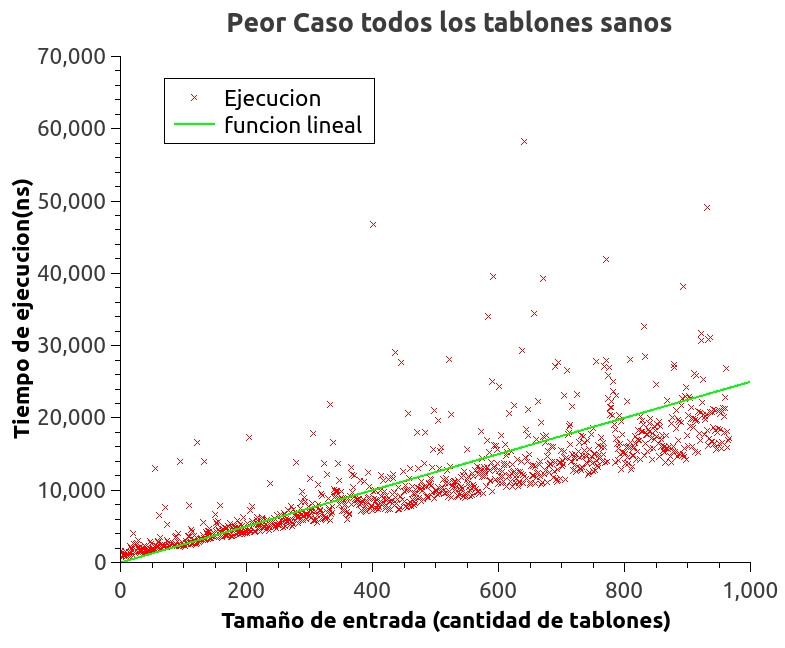
\includegraphics[scale=0.7]{Ej1/sanos.jpg}\\
Como puede verse en el gr�fico su complejidad esta en el orden lineal como puede compararse con la funci�n, en el gr�fico puede observar que algunos casos excede el orden, este ruido se debe a que puede haber ovaciones donde el sistema operativo este realizando otras tareas y afecte el orden de ejecuci�n.

Para el segundo test se realizo un test aleatorio, para poder observar el comportamiento de todos los casos posibles, para esto se crearon 1000 instancias, en las cuales el tama�o del puente fue creciendo de 1 a 1000  y el salto m�ximo es un numero random entre 1 y la cantidad de tablones del puente para poder obtener tambi�n casos que no sean soluci�n, dando comer resultado el siguiente gr�fico.
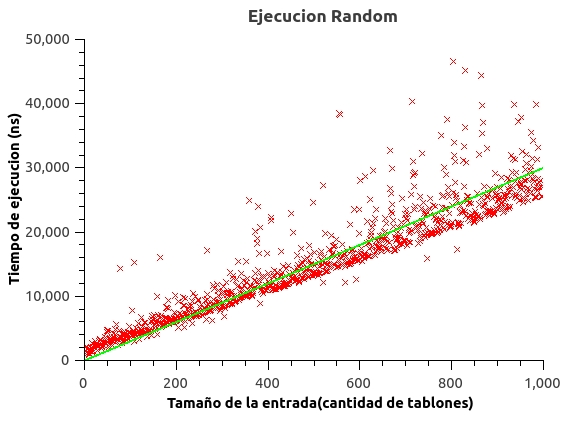
\includegraphics[scale=0.7]{Ej1/Random.jpg}\\

Puede observarse que al igual en el test anterior el orden de complejidad esta en el orden lineal, de esta manera podemos concluir que nuestro algoritmo cumple con los ordenes de complejidad impuestos por el enunciado.

